\documentclass{beamer}
% \setbeamertemplate{navigation symbols}{}
%\setbeamercolor{frametitle}{fg=black,bg=white}
%\setbeamercolor{title}{fg=black,bg=yellow!85!orange}
\usetheme{Boadilla}
\usepackage{makecell}
\usepackage{booktabs}
\usepackage{caption}
\usepackage{amsmath}
\usepackage{epsfig}
\usepackage{epstopdf}
\usepackage{graphicx}
\usepackage{subcaption}
\usepackage{physics}
\usepackage{hyperref}
\hypersetup{
	colorlinks=true,
	linkcolor=blue,
	filecolor=magenta,      
	urlcolor=blue,
}
\usepackage{xcolor}
\usepackage{multirow}
\usepackage{bm}
\usepackage{ragged2e}
\apptocmd{\frame}{}{\justifying}{}

\title[Bayesian Hierarchical Clustering]{Hierarchical Clustering and Bayesian Statistics}
	\author{Mukai Wang}
% \beamersetuncovermixins{\opaqueness<1>{25}}{\opaqueness<2->{15}}
\begin{document}
	
	
	\begin{frame}
		\titlepage
	\end{frame}
	
	\begin{frame}
		\tableofcontents[hideallsubsections]
	\end{frame}

	\section{Hierarchical Clustering}
	
	
	
	
	\begin{frame}{SPADE Clustering}
		\begin{figure}[htbp]
			\centering
			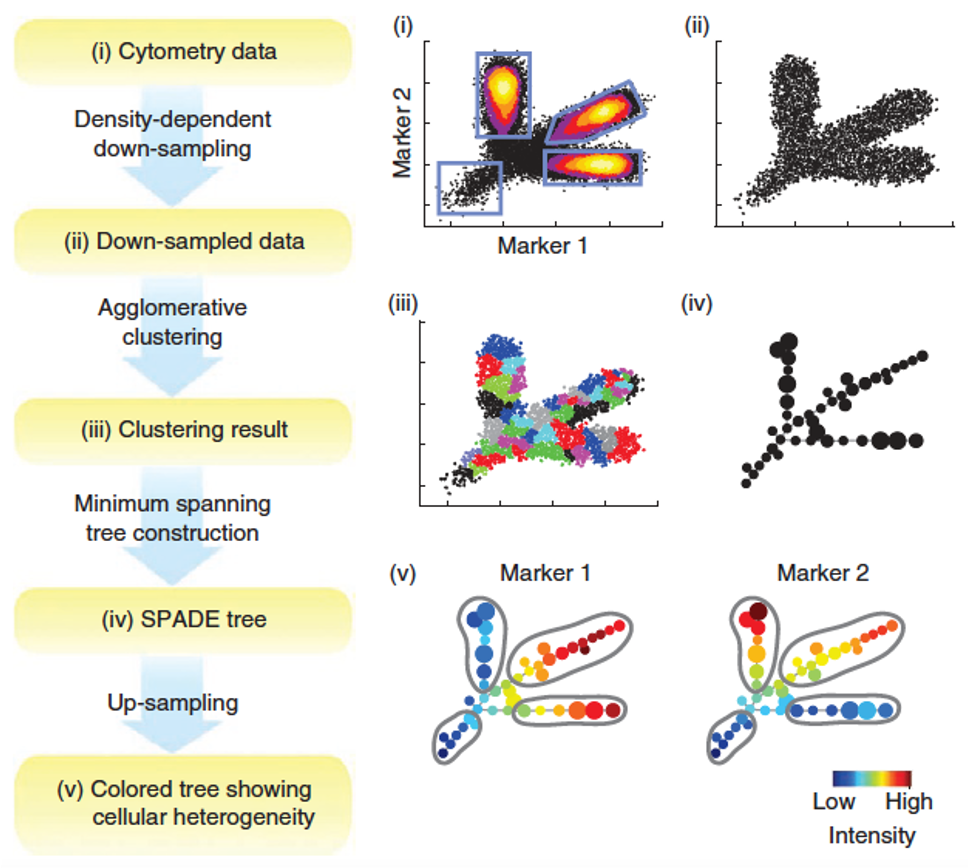
\includegraphics[scale=0.45]{SPADE.png}
			\caption*{Qiu etal \emph{Nature Biotechnology} 2011}
		\end{figure}
	\end{frame}
	
	\begin{frame}{Hierarchical Clustering}
		\begin{figure}[htbp]
			\centering
			\includegraphics[scale=0.33]{ISLRhclust.png}
			\caption*{James etal, \emph{An Introduction to Statistical Learning in R}}
		\end{figure}
	\end{frame}
	\subsection{Agglomerative Clustering}
	\begin{frame}
		\tableofcontents
		[
		currentsection,
		currentsubsection,
		subsectionstyle=show/shaded/hide
		]
	\end{frame}
	
	\begin{frame}{Agglomerative Clustering}
		\begin{columns}
			\begin{column}{0.4\linewidth}
				Our goal is to cluster 7 points into 2 groups.
				\begin{table}[htbp]
					\centering
					\begin{tabular}{ccc}
						\toprule
						Index & X & Y\\
						\midrule
						1 & 2.05 & 1.36\\
						2 & 1.90 & 2.13\\
						3 & 1.49 & 3.12\\
						4 & 2.16 & 1.2\\
						5 & 2.3 & 4.4\\
						6 & 3.27 & 2.9\\
						7 & 3.73 & 3.29\\
						\bottomrule
					\end{tabular}
				\end{table}
			\end{column}
			\begin{column}{0.6\linewidth}
				\begin{figure}[htbp]
					\centering
					\includegraphics[scale=0.6]{scatterplot.pdf}
				\end{figure}
			\end{column}
		\end{columns}
	\end{frame}
	
	\begin{frame}{Agglomerative Clustering}
		To carry out agglomerative clustering, we need to calculate the pairwise distance between each pair of points.
		\[ d(i, j) = \sqrt{(X_i - X_j)^2 + (Y_i - Y_j)^2 }\]
		
		\begin{table}
			\centering
			\begin{tabular}{c|ccccccc}
				&1&2&3&4&5&6&7\\
				\hline
				1&&0.78&1.84&\textcolor{red}{0.20}&3.05&1.96&2.56\\
				2&&&1.07&0.97&2.31&1.57&2.17\\
				3&&&&2.04&1.51&1.79&2.24\\
				4&&&&&3.21&2.03&2.62\\
				5&&&&&&1.79&1.81\\
				6&&&&&&&0.60\\
				7&&&&&&&\\
			\end{tabular}
		\end{table}
	\end{frame}
	
	\begin{frame}{Agglomerative Clustering}
		After finding the smallest pairwise distance, we merge the corresponding two points into one entity.
		\begin{table}[htbp]
			\begin{tabular}{c|cccccc}
				&$\begin{bmatrix}1&4 \end{bmatrix}$ & 2 & 3 & 5 & 6 & 7\\
				\hline
				$\begin{bmatrix}1\\4 \end{bmatrix}$&&0.87&1.94&3.13&2.00&2.59\\
				2&&&1.07&2.31&1.57&2.17\\
				3&&&&1.51&1.79&2.24\\
				5&&&&&1.79&1.81\\
				6&&&&&&\textcolor{red}{0.60}\\
				7&&&&&&\\
			\end{tabular}
		\end{table}
	
		Note that when I calculate the distance between $\{1, 4\}$ and other points, I use the average distance
		\[d\left(\{1, 4\}, 2\right) = \frac{1}{2}\left( d(1,2) + d(1,4) \right) \]
	\end{frame}
	
	\begin{frame}{Agglomerative Clustering}
		\begin{table}[htbp]
			\centering
			\begin{tabular}{c|ccccc}
				&$\begin{bmatrix}1&4 \end{bmatrix}$ & 2&3&5& $\begin{bmatrix}6&7 \end{bmatrix}$\\
				\hline
				$\begin{bmatrix}1\\4 \end{bmatrix}$ & &\textcolor{red}{0.87} &1.94&3.13&2.29\\
				2&&&1.07&2.31&1.87\\
				3&&&&1.51&2.02\\
				5&&&&&1.80\\
				$\begin{bmatrix}6\\7 \end{bmatrix}$&&&&&\\
			\end{tabular}
		\end{table}
	
	\[ d\left(\{1, 4\}, \{6, 7\}\right) =  \frac{1}{4}\left( d(1,6) + d(1,7) + d(4,6) + d(4,7)\right)\]
	\end{frame}
	
	\begin{frame}{Agglomerative Clustering}
		\begin{table}[htbp]
			\begin{tabular}{c|cccc}
				& $\begin{bmatrix}1&2&4 \end{bmatrix}$ &3&5& $\begin{bmatrix}6&7 \end{bmatrix}$\\
				\hline
				$\begin{bmatrix}1\\2\\4 \end{bmatrix}$&&1.65&2.85&2.15\\
				3 &&&\textcolor{red}{1.51}&2.01\\
				5&&&&1.79\\
				$\begin{bmatrix}6\\7 \end{bmatrix}$&&&&\\ 
			\end{tabular}
		\end{table}
	\end{frame}
	
	\begin{frame}{Agglomerative Clustering}
		\begin{table}[htbp]
			\begin{tabular}{c|ccc}
				&$\begin{bmatrix}1&2&4 \end{bmatrix}$ & $\begin{bmatrix}3&5 \end{bmatrix}$&$\begin{bmatrix}6&7 \end{bmatrix}$\\
				\hline
				$\begin{bmatrix}1\\2\\4 \end{bmatrix}$ &&2.25&2.15\\
				$\begin{bmatrix}3\\5 \end{bmatrix}$ &&&\textcolor{red}{1.91}\\
				$\begin{bmatrix}6\\7 \end{bmatrix}$ &&&\\
			\end{tabular}
		\end{table}
	At this point, we know that $\{3,5\}$ and $\{6,7\}$ will first be merged, then all the points will be merged together.
	\end{frame}
	
	\begin{frame}{Agglomerative Clustering}
		\begin{figure}[htbp]
			\begin{subfigure}[b]{0.45\columnwidth}
				\centering
				\includegraphics[scale=0.5]{agglodendrogram.pdf}
			\end{subfigure}
			\hfill
			\begin{subfigure}[b]{0.45\columnwidth}
				\centering
				\includegraphics[scale=0.47]{aggloresult.pdf}
			\end{subfigure}
		\end{figure}
	\end{frame}
	
	\subsection{Divisive Clustering}
	\begin{frame}
		\tableofcontents
		[
		currentsection,
		currentsubsection,
		subsectionstyle=show/shaded/hide
		]
	\end{frame}
	
	\begin{frame}{Divisive Clustering}
		\begin{columns}
			\begin{column}{0.4\linewidth}
				\begin{table}[htbp]
					\centering
					\begin{tabular}{ccc}
						\toprule
						Index & X & Y\\
						\midrule
						1 & 2.05 & 1.36\\
						2 & 1.90 & 2.13\\
						3 & 1.49 & 3.12\\
						4 & 2.16 & 1.2\\
						5 & 2.3 & 4.4\\
						6 & 3.27 & 2.9\\
						7 & 3.73 & 3.29\\
						\bottomrule
					\end{tabular}
				\end{table}
			\end{column}
			\begin{column}{0.6\linewidth}
				\begin{figure}[htbp]
					\centering
					\includegraphics[scale=0.6]{scatterplot}
				\end{figure}
			\end{column}
		\end{columns}
	\end{frame}

	\begin{frame}{Divisive Clustering}
		
		First calculate the average distance to other points for each point. For example, the average distance of point 1 with other points is
		\[(0.78+1.84+0.20+3.05+1.96+2.56)/6=1.73 \]
		\begin{table}[htbp]
			\centering
			\begin{tabular}{cc}
				\toprule
				Point & \makecell{Average Distance \\ to Other Points}\\
				\midrule
				1 & 1.73 \\
				2 & 1.48 \\
				3 & 1.75 \\ 
				4 & 1.84 \\
				5 & \textcolor{red}{2.28}  \\
				6 & 1.62 \\
				7 & 2.00 \\
				\bottomrule
			\end{tabular}
		\end{table}
		
	\end{frame}
	
	\begin{frame}{Divisive Clustering}
		We separate out point 5 to be a new cluster. Then we need to decide if we want to move other points from $\{1,2,3,4,6,7 \}$ to the new cluster. We calculate the average distance to the remaining points and the average distance to the new cluster of "splinter points".
		
		\begin{table}[htbp]
			\begin{tabular}{cccc}
				\toprule
				Point & \makecell{Average Distance \\ to Remaining Points} & \makecell{Average Distance \\ to Splinter Points} & Difference\\
				\midrule
				1& 1.47 & 3.05 & -1.579\\
				2& 1.31 & 2.31 & -0.995\\
				3& 1.80 & 1.51 & \textcolor{red}{0.284}\\
				4& 1.57& 3.21 & -1.636\\
				6& 1.59 & 1.79 & -0.196\\
				7& 2.04&  1.81 & 0.229\\
				\bottomrule
			\end{tabular}
		\end{table}
	\end{frame}

	\begin{frame}{Divisive Clustering}
		We add point 3 to the new cluster $\{3, 5\}$, then we check the rest of the points $\{1,2,4,6,7\}$.
		\begin{table}[htbp]
			\begin{tabular}{cccc}
				\toprule
				Point & \makecell{Average Distance \\ to Remaining Points} & \makecell{Average Distance \\ to Splinter Points} & Difference\\
				\midrule
				1& 1.37 & 2.45 & -1.08\\
				2& 1.37 & 1.69 & -0.32\\
				4& 1.45& 2.62 & -1.17\\
				6& 1.54 & 1.79 & -0.25\\
				7& 1.99&  2.03 & -0.04\\
				\bottomrule
			\end{tabular}
		\end{table}
		We notice that all the points are more \emph{comfortable} with the current group than joining the new cluster, therefore we stop here.
	\end{frame}
	
	\begin{frame}{Comments}
		We realize that the agglomerative clustering and the divisive clustering provided different results.
		\begin{figure}[htbp]
			\begin{subfigure}[b]{0.45\columnwidth}
				\centering
				\includegraphics[scale=0.5]{aggloresult}
				\subcaption*{Agglomerative Clustering}
			\end{subfigure}
			\hfill
			\begin{subfigure}[b]{0.45\columnwidth}
				\centering
				\includegraphics[scale=0.5]{divresult}
				\subcaption*{Divisive Clustering}
			\end{subfigure}
		\end{figure}
	\end{frame}
	
	\begin{frame}{Comments}
		Neither of them is correct. The data are generated from two 2D Gaussian distributions, one centered at $(2,2)$ and the other centered at $(3,3)$.
		\begin{figure}[htbp]
			\begin{subfigure}{0.48\columnwidth}
				\centering
				\includegraphics[scale=0.27]{2DGaussian.png}
			\end{subfigure}
			\hfill
			\begin{subfigure}{0.48\columnwidth}
				\centering
				\includegraphics[scale=0.47]{datagen}
			\end{subfigure}
		\end{figure}
	\end{frame}
	
	
	\begin{frame}{Comments}
		\begin{itemize}
			\item Hierarchical clustering has great potential of grouping subjects effectively.
			\item Different hierarchical clustering procedures have their own merits and provide different feasible results.
			\begin{itemize}
				\item Agglomerative clustering is simpler than divisive clustering.
				\item Divisive clustering is more efficient if we don't need a complete hierarchy.
			\end{itemize}
			\item Clustering subjects has uncertainty. It's crucial to quantify the uncertainty for medical experts to make informed decision.
		\end{itemize}
	\end{frame}
	
	\section{Bayesian Statistics}
	\subsection{Basic Idea of Bayesian Statistics}
		\begin{frame}
		\tableofcontents
		[
		currentsection,
		currentsubsection,
		subsectionstyle=show/shaded/hide
		]
	\end{frame}

	\begin{frame}{Example: Inference about a Genetic Status}
		Hemophilia is a genetic disease that exhibits X-chromosome-linked recessive inheritance. Consider a woman who is not affected but has an affected brother and unaffected parents. We need an estimate of the chance this woman being a carrier as accurate as possible.
		\begin{figure}[htbp]
			\centering
			\includegraphics[scale=0.6]{GeneticsTree.pdf}
		\end{figure}
	\end{frame}

	\begin{frame}{Example: Inference about a Genetic Status}
		The current information tells us that the probability of this woman being a carrier ($\theta=1$) versus not being a carrier ($\theta=0$) is the same, namely $P(\theta=1) = P(\theta=0) = 1/2$
		
		\pause
		Now we have additional information that this woman has two sons, and neither of them is affected. We can use this information to update our estimate of $\theta$. \pause Let's use $y_1$ and $y_2$ to denote whether her two sons are affected. If the woman is a carrier, then the chance of her sons being unaffected is
		
		$$ P(\left. y_1=0, y_2=0 \right\vert \theta=1) = 0.5\times 0.5=0.25 $$
		
		\pause
		If the woman is not a carrier, then the chance of her sons being unaffected is
		
		$$ P(\left. y_1=0, y_2=0 \right\vert \theta=0) =1 \times 1=1 $$
	\end{frame}

	\begin{frame}{Example: Inference about a Genetic Status}
		The new information help us update the probability that this woman being a carrier
		\small
		\begin{align*}
			&\quad P(\left.\theta=1 \right\vert y_1, y_2) \\
			&= \frac{P(\left. y_1=0, y_2=0 \right\vert \theta=1) P(\theta=1)}{P(\left. y_1=0, y_2=0 \right\vert \theta=1) P(\theta=1) + P(\left. y_1=0, y_2=0 \right\vert \theta=0) P(\theta=0)}\\
			&=\frac{0.25\times 0.5 }{0.25\times 0.5 + 1\times 0.5} = 0.2
		\end{align*}
		
		The fact that the woman's sons are healthy make us believe that the woman is unlikely to be a carrier of hemophilia.
	\end{frame}	
	
	\begin{frame}{Bayesian Statistics Philosophy}
	\small
		\begin{table}[htbp]
			\centering
			\renewcommand{\arraystretch}{2.4}
			\begin{tabular}{cc}
			\toprule
			& Hemophilia Genetics\\
			\midrule
			\makecell{Prior Belief about \\ unobserved quantity of interest} & Mom's chance of being a carrier \\
			\makecell{Connection Between Observed \\ and Unobserved Quantity} & Sons' disease probability given Mom's status\\
			\makecell{Observed Data} & Disease Status of Sons \\
			\makecell{Posterior Inference} & \makecell{Updated chance of  Mom being a carrier} \\
			\bottomrule
			\end{tabular}
		\end{table}
	\end{frame}

	\subsection{Gaussian Mixture Model with Fixed Number of Clusters}
		\begin{frame}
		\tableofcontents
		[
		currentsection,
		currentsubsection,
		subsectionstyle=show/shaded/hide
		]
	\end{frame}

	\begin{frame}{Example: Iris Dataset}
		American Botanist Edgar Anderson measured the sepal length, sepal width, petal length and petal width of three different kinds of Iris flower species. Here we aim to carry out clustering based on petal length and petal width.
		\begin{figure}[htbp]
		\centering
		\includegraphics[scale=0.55]{iris.pdf}
		\end{figure}
	\end{frame}

	\begin{frame}{Bayesian Statistics Philosophy}
			\begin{table}[htbp]
			\centering
			\renewcommand{\arraystretch}{2.4}
			\begin{tabular}{cc}
			\toprule
			& Iris Clustering\\
			\midrule
			\makecell{Prior Belief about \\ unobserved quantity of interest} & \makecell{Number of Clusters, \\cluster proportion \\ and distribution in each cluster   } \\
			\makecell{Connection Between Observed \\ and Unobserved Quantity} & \makecell{ Distribution landscape of\\ petal length and width} \\
			\makecell{Observed Data} & Petal lengths and widths \\
			\makecell{Posterior Inference} & \makecell{ Updated cluster size, \\ cluster proportion and \\ and distribution in each cluster } \\
			\bottomrule
			\end{tabular}
		\end{table}
	\end{frame}

	\begin{frame}{Gaussian Mixture Model with Fixed Cluster Number}
		In this section we assume that we already know there are three clusters.
		\begin{figure}[htbp]
		\begin{subfigure}[b]{0.48\columnwidth}
			\centering
			\includegraphics[scale=0.40]{2DGMM.png}
			\subcaption{Gaussian Mixture Distribution}
		\end{subfigure}
		\hfill
		\begin{subfigure}[b]{0.48\columnwidth}
			\centering
			\includegraphics[scale=0.12]{dirichletdemo}
			\subcaption{Dirichlet distribution for three categories}
		\end{subfigure}
			\end{figure}
	\end{frame}

	\begin{frame}{Prior Distribution Setup}
		\begin{itemize}
			\item We use a gaussian mixture distribution to describe the distribution landscape of petal length and widths for all the flowers.
			$$ \bm{y} \sim \sum_{j=1}^{3}\pi_j \mathcal{N}(\bm{\mu}_j, \Sigma_{j}) $$
			\item To express our prior beliefs about cluster proportion, cluster mean and cluster variance, we impose some statistical distributions on them as well.
			\begin{align*}
				\bm{\mu}_j & \sim \mathcal{N}(\bar{\bm{\mu}}, c\Sigma_j)\quad \text{for j=1,2,3}\\
				\Sigma_j & \sim \mathcal{IW}(\nu, V) \quad \text{for j=1,2,3} \\
				\begin{bmatrix} \pi_1 & \pi_2 & \pi_3 \end{bmatrix} & \sim \text{Dirichlet}(\begin{bmatrix} a_1 & a_2 & a_3 \end{bmatrix})
			\end{align*}
			\item We need to provide a number for $\bar{\bm{\mu}}$, $c$, $\nu$, $V$ and $\begin{bmatrix} a_1 & a_2 & a_3 \end{bmatrix}$.
		\end{itemize}
	\end{frame}

	\begin{frame}{Posterior Inference}
		Through some nontrivial computation, we can get a posterior distribution for the cluster mean $\bm{\mu}_1$, $\bm{\mu}_2$, $\bm{\mu}_3$ and the cluster variance $\Sigma_1$, $\Sigma_2$ and $\Sigma_3$. I take the mean value from the posterior distributions and visualize them below.
		\begin{figure}[htbp]
		\begin{subfigure}[b]{0.48\columnwidth}
			\centering
			\includegraphics[scale=0.42]{iris_postmean}
			\subcaption{Posterior GMM Components}
		\end{subfigure}
		\hfill
		\begin{subfigure}[b]{0.48\columnwidth}
			\centering
			\includegraphics[scale=0.42]{iris_pred}
			\subcaption{Cluster Prediction}
		\end{subfigure}
			\end{figure}
		
	\end{frame}


	\subsection{Gaussian Mixture Model with Flexible Number of Clusters}
		\begin{frame}
		\tableofcontents
		[
		currentsection,
		currentsubsection,
		subsectionstyle=show/shaded/hide
		]
	\end{frame}

	\begin{frame}{Dirichlet Process(Chinese Restaurant Process)}
		Can we estimate the number of clusters and the cluster parameters(mean, variance etc) simultaneously? Some statisticians drew inspiration from 
		\href{https://topicmodels.west.uni-koblenz.de/ckling/tmt/crp.html?parameters=10&dp=1}{Chinese restaurant process} and came up with a statistical algorithm that solves the problem.
		\pause
		
		\begin{enumerate}
			\item We start with the first flower and put it into a cluster. The cluster parameter (mean, variance etc) is randomly sampled from the posterior distribution taking into account our prior belief and the petal length and width of this first flower.
			\pause
			\item As we introduce the second flower, we can choose to assign it to the same cluster as the first flower(share the same cluster parameter) or we choose to set up a new cluster for this second flower with its own cluster parameters. The decision is stochastic, and it's influenced by the resemblance between the second flower and the first flower.
			\pause
			\item We continue this process and assign new flowers either to one of the existing clusters, or allocate a new cluster for the new member.
			\pause
			\item We repeat this procedure many times. 
		\end{enumerate}
	\end{frame}

	\begin{frame}{GMM with Dirichlet Process}
		I loop through the 150 data points 2000 times. Among the last 1000 iterations,
		\begin{columns}
			\begin{column}{0.3\textwidth}
				
				\begin{table}[htbp]
					\small
					\centering
					\begin{tabular}{cc}
						\toprule
						Clusters & Iterations\\
						\midrule
						2 & 845\\
						3 & 137 \\
						4& 8 \\
						5& 1\\
						\bottomrule
					\end{tabular}
				\end{table}
			\end{column}
			\begin{column}{0.7\textwidth}
				\begin{figure}[htbp]
					\centering
					\includegraphics[scale=0.52]{iris_dir_pred.pdf}
				\end{figure}
			\end{column}
		\end{columns} 
	\end{frame}

	\begin{frame}{What's Next?}
		\begin{itemize}
			\item Hierarchical clustering is a promising clustering method, but we need to quantify the uncertainty of this algorithm to develop a deeper understanding.
			\item Bayesian statistics is a popular philosophy for quantifying uncertainty.
			\item For the next step, I aim at applying Bayesian statistics idea to explain the uncertainty of hierarchical clustering.
		\end{itemize}
	\end{frame}

	\section{Diffusion Tree Prior}
	\begin{frame}{Diffusion Tree Process}
	\small
			Similar to Dirichlet process, Diffusion tree process also treats the distribution of data points as generated from an imaginary process.

The first point is imagined to be a destination of a brownian motion for $t=1$ from point 0.

The second point follows the same path as the first point until it breaks away at some point.

			\begin{figure}[htbp]
				\centering
				\includegraphics[scale=0.3]{DTmotive.png}
			\end{figure}
	\end{frame}

	\begin{frame}{Diffusion Tree Process}
	\begin{figure}[htbp]
			\centering
			\includegraphics[scale=0.25]{simplifiedmotive.png}
		\end{figure}
		
		Denote $A(t) = \int_{0}^{t}a(u)du$ as the probability of a point splitting from the original path by time $t$, and that the probability of splitting from a path that has been traversed by $m$ points within an infinitesimal interval to be $a(t)dt/m$. $a(t)$ is commonly chosen to be in the form $c/(1-t)$ or $b+d/(1-t)^2$.
		
	\end{frame}

	\begin{frame}{Diffusion Tree Process}
	
	\begin{figure}[htbp]
			\centering
			\includegraphics[scale=0.2]{simplifiedmotive.png}
		\end{figure}	
	
	The probability density is the product of two factors. The tree structure factor is
	$$ e^{-A(t_a)} a(t_a) \times e^{-A(t_b)/2}(a(t_b)/2)\times e^{-A(t_b)/3}(1/3)e^{A(t_b) - A(t_c)}a(t_c) $$
	The data factor is
	\begin{align*}
	\small
		N(\left.x_b \right\vert 0, \sigma^2 t_b) & \times N(\left.x_a \right\vert x_b, \sigma^2 (t_a - t_b)) \times N(\left.x_1 \right\vert x_a ,\sigma^2 (1-t_a))\\ & \times N(\left.x_2 \right\vert x_a, \sigma^2 (1-t_a)) 
		\times N(\left.x_c \right\vert x_b, \sigma^2 (t_c - t_b))\\ & \times N(\left.x_3 \right\vert x_c ,\sigma^2 (1-t_c)) \times N(\left.x_4 \right\vert x_c, \sigma^2 (1-t_c))
	\end{align*}
	\end{frame}

	\begin{frame} {Diffusion Tree Process}
		To generate a number of diffusion tree samples and understand the uncertainty of hierarchical clustering, we repeatedly take out a node and try to put it back into the tree.
		
		\begin{figure}[htbp]
			\centering
			\includegraphics[scale=0.32]{DTsampling.png}
		\end{figure}
	\end{frame}

	\begin{frame}{Further Reading}
		\begin{itemize}
			\item \href{https://www.nature.com/articles/nbt.1991}{Extracting a cellular hierarchy from high-dimensional
			cytometry data with SPADE} by Qiu etal
			\item \href{https://www.statlearning.com/}{Introduction to Statistical Learning} by James, Witten, Hastie and Tibshirani
			\item \href{https://onlinelibrary.wiley.com/doi/book/10.1002/9780470316801}{Finding Groups in Data} by Kaufman and Rousseeuw
			\item \href{http://www.stat.columbia.edu/~gelman/book/}{Bayesian Data Analysis} by Gelman etal
			\item \href{https://www.jstor.org/stable/2291069?seq=1}{Bayesian Density Estimation and Inference Using Mixtures} by Escobar and West
			\item \href{https://www.jstor.org/stable/1390653?seq=1}{Markov Chain Sampling Methods for Dirichlet Process Mixture Models} by Neal
		\end{itemize}
	\end{frame}


\end{document}